\let\negmedspace\undefined
\let\negthickspace\undefined
\documentclass[journal]{IEEEtran}
\usepackage[a5paper, margin=10mm, onecolumn]{geometry}
%\usepackage{lmodern} % Ensure lmodern is loaded for pdflatex
\usepackage{tfrupee} % Include tfrupee package

\setlength{\headheight}{1cm} % Set the height of the header box
\setlength{\headsep}{0mm}     % Set the distance between the header box and the top of the text

\usepackage{gvv-book}
\usepackage{gvv}
\usepackage{cite}
\usepackage{amsmath,amssymb,amsfonts,amsthm}
\usepackage{algorithmic}
\usepackage{graphicx}
\usepackage{textcomp}
\usepackage{xcolor}
\usepackage{txfonts}
\usepackage{listings}
\usepackage{enumitem}
\usepackage{mathtools}
\usepackage{gensymb}
\usepackage{comment}
\usepackage[breaklinks=true]{hyperref}
\usepackage{tkz-euclide} 
\usepackage{listings}
% \usepackage{gvv}                                        
\def\inputGnumericTable{}                                 
\usepackage[latin1]{inputenc}                                
\usepackage{color}                                            
\usepackage{array}                                            
\usepackage{longtable}                                       
\usepackage{calc}                                             
\usepackage{multirow}                                         
\usepackage{hhline}                                           
\usepackage{ifthen}                                           
\usepackage{lscape}
\usepackage{circuitikz}
\tikzstyle{block} = [rectangle, draw, fill=blue!20, 
    text width=4em, text centered, rounded corners, minimum height=3em]
\tikzstyle{sum} = [draw, fill=blue!10, circle, minimum size=1cm, node distance=1.5cm]
\tikzstyle{input} = [coordinate]
\tikzstyle{output} = [coordinate]

\begin{document}

\bibliographystyle{IEEEtran}
\vspace{3cm}

\title{1.5.1}
\author{EE25BTECH11051 - Shreyas Goud Burra}
\maketitle
% \newpage
% \bigskip
{\let\newpage\relax\maketitle}

\renewcommand{\thefigure}{\theenumi}
\renewcommand{\thetable}{\theenumi}
\setlength{\intextsep}{10pt} % Space between text and floats


\numberwithin{equation}{enumi}
\numberwithin{figure}{enumi}
\renewcommand{\thetable}{\theenumi}


\textbf{Question}

Find the ratio in which the Y axis divides the line segment joining the points (6, -4)
and (-2, -7). Also find the point of intersection.

\solution \\

Let us solve the given equation theoretically and then verify the solution computationally. \\

Assume the two points to be position vectors $\textbf{A} = \myvec{6 \\ -4}$ and $\textbf{B} = \myvec{-2 \\ -7}$
To find the ratio in which the Y axis divides the line segment. We can use the section formula

\begin{align}
    \textbf{C} = \brak{\frac{\frac{m}{n}A+B}{\frac{m}{n}+1}}
    \label{0.1}
\end{align}


Here, $\textbf{C}$ is the vector on the Y axis that intersects the line segment joining the position vectors $\textbf{A}$ and $\textbf{B}$ and divides it in the ratio of $m:n$, where m and n are integers in their lowest form.\\ 

Here we can assume some constant $k=\frac{m}{n}$. This gives us

\begin{align}
    \textbf{C} = \brak{\frac{kA+B}{k+1}}
    \label{0.2}
\end{align}

We know that the point which divides the line segment lies on the Y axis and therefore its x coordinate is zero.\\

We can write \textbf{C} as 

\begin{align}
    \mathbf{C} = \myvec{0 \\ y}
    \label{0.3}
\end{align}

Where $y$ is the y coordinate of the point of intersection of the Y axis and the line segment AB.\\
We know that these three points are collinear, so by using rank method we get. Rank of matrix 

\begin{align}
    \textbf{P} = (\textbf{B}-\textbf{A} \text{ } \textbf{C}-\textbf{A}) = 1 \\
    \implies \text{Rank of } \myvec{-8 & -6 \\ -3 & y+4} = 1
    \label{0.4}
\end{align}
On applying row transformations

$$ R_2 \rightarrow R_2 - \frac{3}{8}R_1$$

\begin{align}
    \textbf{C} = \myvec{-8 & -6 \\ 0 & y+\frac{25}{4}}\\
\end{align}

If rank = 0

\begin{align}
    \implies y+\frac{25}{4} = 0\\
    y = -\frac{25}{4}
\end{align}



We get the same result by plotting the graph

\begin{figure}[H]
    \centering
    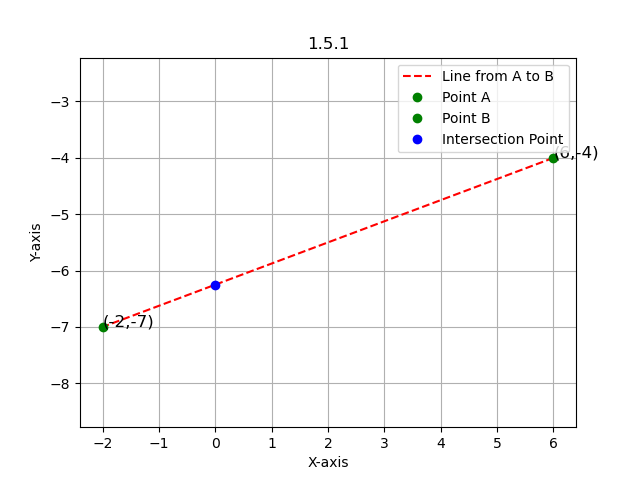
\includegraphics[width=1.1\columnwidth]{figs/fig1.png}
    \caption{2D Plot}
    \label{fig:placeholder}
\end{figure}



\end{document}
